\section{High level Architecture}
\label{fig:architecture_diagram}
\begin{figure}[t]
\centering
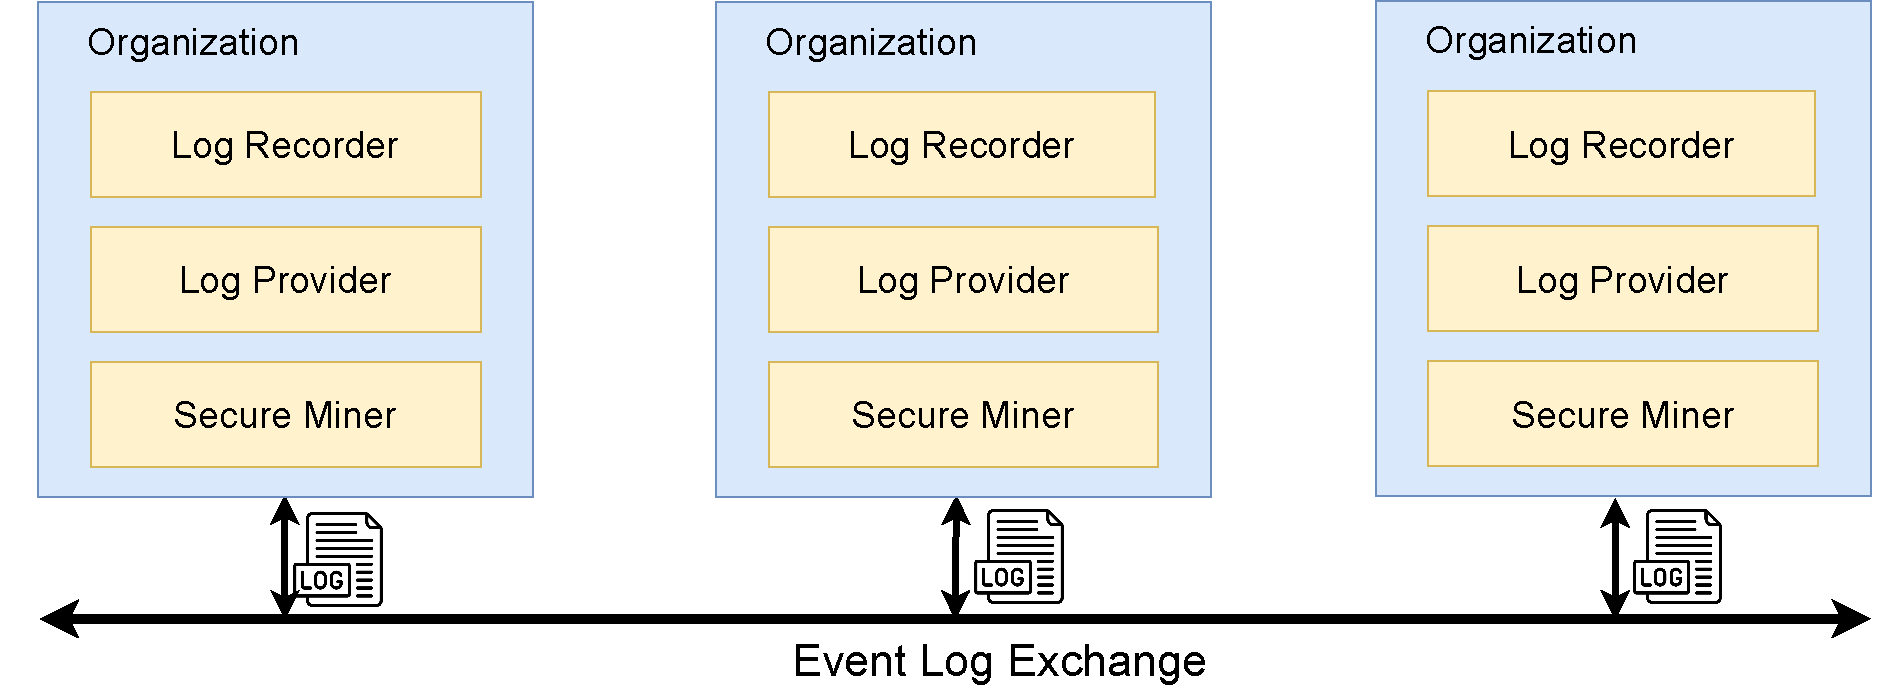
\includegraphics[width=11cm]{content/figures/architecture_diagram.pdf}
\caption{High-level architectural overview of the framework.}
\label{fig:implementation}
\end{figure}
In the following section we present the high level architecture underlying our solution. Therefore, we take into account each component individually. Once introduced the architecture, we provide an overview on the main interactions taking place between the introduced components.
\subsection{Main components}
Our architecture involve networks of nodes controlled by different \texttt{Organization}s exchanging their event logs. \texttt{Organization}s in the same network collaborate to reach a common objective sharing one or more business processes. Each organization is associated with  The Hospital and Specialized Clinic, mentioned in the running example, provide an example of partner organizations.

In \cref{fig:architecture_diagram}, we propose an high level schematization of our solution. Each organization embeds three main components: the \texttt{ERP Interface}, the \texttt{Log Provider} and the \texttt{Trusted Miner}. %collects the logic to interact with the Environmental Management System (EMS) of the organization. The \texttt{Log Provider} component deliver on-demand data to partner organization's systems. The \texttt{Trusted Miner} executes process mining algorithms inside the \texttt{Trusted Execution Environment} using event log retrieved from partner organizations.
In the next paragraph, we address the newly mentioned components.
\subsubsection{ERP Interface}
The \texttt{ERP Interface} collects the logic to interact with the Enterprise Resource Planning (ERP) system  of the \texttt{Organization}. ERP systems helps organizations to
handle business processes including accounting and resource management. The mantainance of event logs is one of the many tasks performed by these systems. In our architecture, we generalize the interaction with these systems through the \texttt{ERP Interface}. The \texttt{ERP Interface} provide the local \texttt{Log Provider} and \texttt{Trusted Miner} access to event logs generated inside the \texttt{Organization}.
\subsubsection{Log Provider}
The \texttt{Log Provider} component deliver on-demand data to \texttt{Trusted Miner}s belonging to partner \texttt{Organization}'s. It handle event log request through access control methodologies, thanks to which the identity of the sender is determined and the access to the resource is decided.

\texttt{Log Provider}s authenticate event log requests using asymetric encryption methodologies. Through the latter, \texttt{Log Provider}s verifiy parameters embedded in the data request. The goal of the authentication procedure is to extract the public key stating the identity of the sender \texttt{Trusted Miner}. In order to deliver data, the \texttt{Log Provider} retrieve the local event log communicating with the \texttt{ERP Interface} of the \texttt{Organization}.

Remote Attestation and Log Segmentation are crucial procedures handled by the \texttt{Log Provider} during the provision process. Through Remote Attestation, \texttt{Log Provider}s verify that the \texttt{Trusted Miner} that has generated the log request  is: (i) a known software object running inside a trusted execution environment; (ii) controlled by a partner \texttt{Organization} that has rights to access the event log. We named Log Segementation the process through which \texttt{Log Provider}s split the event log to be delivered in sub-log of smaller size.

Our architecture enables the adoption of multiple web protocols appropriated for the \texttt{Log Provider} implementation. HTTP\footnote{HTTP protocol \url{https://httpwg.org/specs/rfc9110.html}, accessed \today.}, FTP and Gopher are some of the suitable candidate for this task.
\label{fig:trusted_miner}
\begin{figure}[t]
\centering
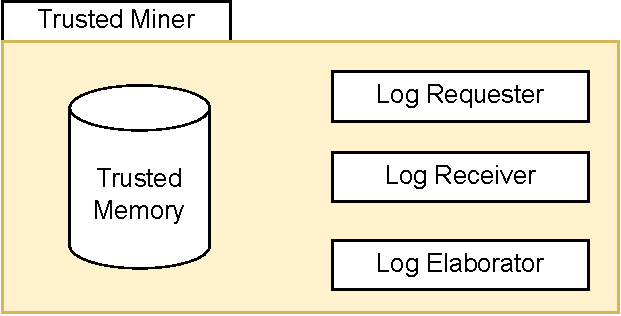
\includegraphics[width=7cm]{content/figures/Trusted_miner.pdf}
\caption{Focus on Trusted Miners running inside Trusted Execution Environments}
\label{fig:implementation}
\end{figure}
\subsubsection{Trusted Miner}
In our solution, \texttt{Trusted Execution Environments} are the key technologies that shelter external event logs inside an \texttt{Organization}'s system by preserving data confidentiality and integrity. The \texttt{Trusted Miner} executes process mining algorithms inside the \texttt{Trusted Execution Environment} using local event log alongside event log retrieved from partner organizations. In \cref{fig:trusted_miner}, we show an high level schematization of \texttt{Trusted Miner}s. As shown in the image, we distinguish four different modules: The \texttt{Trusted Memory}, \texttt{Log Requester}, \texttt{Log Receiver}, and \texttt{Log Elaborator}.

\subsection{Workflow}
\subsubsection{Initialization}
\subsubsection{Data Exchange}
\subsubsection{Data Elaboration}



